% !TeX root = ../main.tex
% Add the above to each chapter to make compiling the PDF easier in some editors.

\section{Monoscopic Far-Field Rendering}
\subsection{Theory}
Monoscopic Far-Field Rendering (MFFR) is a curious approach strongly aligning with an inherent property of many optimizations in the field of rendering and real-time computing in general, which is the property of trading accuracy for speed. MFFR is a topic brought up again in the early days of Rift CV1's retail launch by [TODO: Oculus? Epic? check timeframe] at developer keynotes. \\
Understanding the concept requires some explanation of the technical and visual background. Proper depth perception of the human eye relies on the slight spatial distance between both eyes as each eye sees a slightly different angle of a given object. This difference in perceived angle is called stereo separation [TODO: word this more scientifically?] and without it, the brain has a hard to impossible time determining the depth of and at which a certain object or surface lies. Regular stereo rendering obviously recreates this separation correctly when rendering the two virtual eyes at their respective spatial offset from the HMD center - given correct projection and view matrices and accurate world scale at least. 
However, and that's one aspect MFFR exploits, as distance grows, stereo separation shrinks. In infinity, separation would be infinitely small, but even at more reasonable distances separation becomes so small that even with good vision it becomes hard to properly judge depth unless the object is large. This of course also holds true for rendered stereoscopy, but an additional limit is the pixel density of the output displays. What this means is that at a certain distance from the virtual camera, stereo separation will shrink to less than a full screen space pixel once projected. Obviously if the difference can physically not be displayed by the HMD, it seems a waste of resources to still render both eyes. \\
Mono Far-Field Rendering thus opts to skip the second view during rendering of the name-giving far field of objects. The hope here is that only rendering a single view past a certain distance reduces rendering load without the user noticing the theoretical loss in accuracy. 
This approach has caveats unfortunately. For one, the value at which a field split - the distance at which the stereo rendering is cut off and followed by only mono rendering - will depend on the individual user, their quality of vision and spatial recognition [TODO: better word for that]. It will also potentially depend on the resolution of the used headset given the user's vision is good enough to not deteriorate before that point. \\
Note here, this thesis will not explore these constraints of MFFR further than approximate values used for testing as time does not allow more. \\
MFFR has been implemented by Oculus LLC and Epic Games Inc in Unreal Engine 4 at some point and was recommended for example for certain types of mobile VR experiences with very limited GPU power, but curiously has been removed from the engine in update 4.20 without further explanation. An odd decision surely, as Oculus LLC developer blog posts prior to the removal indicated continued optimization efforts such as added compatibility with UE4's multiview path. 

[TODO: illustration]
\begin{figure}[htpb]
  \centering
  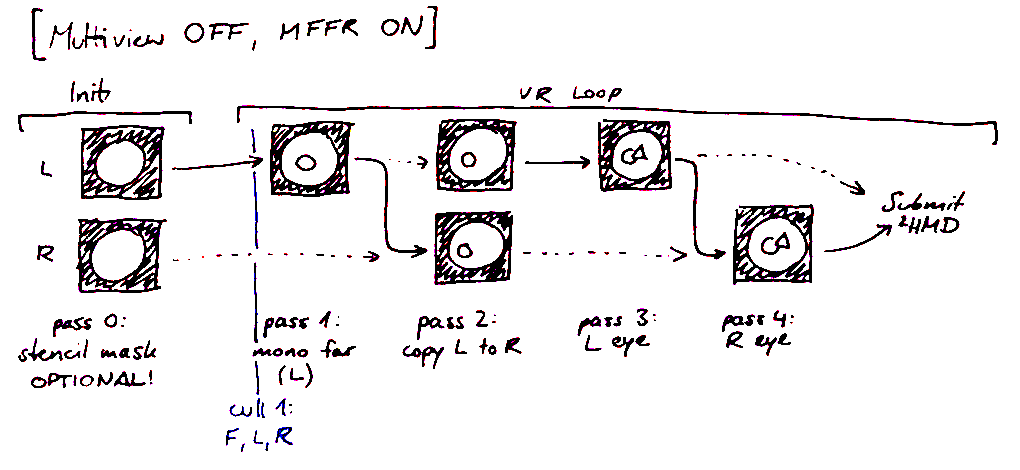
\includegraphics[width=0.9\textwidth]{pictures/flowchart_mffr}
  \caption{[TODO: Monoscopic Far-Field rendering flowchart]} \label{fig:flowchart_mffr}
\end{figure}

\subsection{Estimated impact}
The makeup of the scene itself will also affect effectiveness of the solution. As cautioned by Oculus LLC in their developer reference on Mono Far-Field Rendering [TODO: src], there is a certain baseline overhead simply for enabling the additional render pass necessary for the monoscopic image and the associated context switches. Furthermore only scenes with a significant of distant geometry beyond the field split distance will benefit from the optimization, as obviously the second view workload can only be saved for objects that would be contained within that second pass. 
[TODO]

\subsection{Implementation specifics}
Implementing Mono Far-Field Rendering into Tachyon - or any renderer for that matter - requires care and a number of changes. In this case, the plan was to do MFFR as illustrated in \autoref{fig:flowchart_mffr}, by way of two render passes but only a single framebuffer. In the first step of each VR frame, a monoscopic render pass would render the far clip volume into the index 0 layer of the framebuffer [TODO: ...can Vulkan be set to write pixels into two buffers at the same time?]. The next step would copy that layer to index 1 as well. In the final step then the regular stereoscopic render commands would be executed with reduced near field clip volume. The goal of this approach is to reduce memory operations and locality to a minimum and also avoid more costly compositing methods. While the general approach sounds straight-forward, implementing it in a Vulkan renderer is no trivial task and required the following changes to the renderer: 
\begin{itemize}
\item for the virtual camera, a field split distance parameter is introduced and an additional frustum is added - the stereo frusta then cover the volume from near plan to split plane while the far field frustum covers split plane to far plane
\item the frustum culling procedure is altered to write the far frustum's resulting draw commands into a separate set instead of merging them into one (as would happen for regular multifrustum culling in Tachyon)
\item at initialization time of the VR render target, an additional render pass is created for monoscopy, with the main difference compared to the VR render pass being that it foregoes the multiview extension
\item add an additional set of Vulkan \codeword{VkCommandBuffer}s into which the draw commands of the far frustum cull set are to be recorded
\item add an additional set of \codeword{VkSemaphore}s to synchronize the two render passes and create them in \codeword{CreateSyncObjects()} during initialization
\item add an additional \codeword{VkCommandBuffer} for the layer copy operation
\item at initialization time of the VR render target, pre-record this copy command buffer so it can be reused every frame; this recording includes transitioning the layout of both the color and depth image from \codeword{VK_IMAGE_LAYOUT_TRANSFER_SRC_OPTIMAL} to \codeword{VK_IMAGE_LAYOUT_GENERAL}, \codeword{vkCmdCopyImage(...)} both images' layer 0 to layer 1 and then transition the layouts in reverse again
\item in the per-frame recording procedure of the VR render target, \codeword{RecordCommandBuffers(...)}, the entire structure of begin and end of command buffers and render pass and per-pipeline \codeword{RecordDrawCommand(...)} calls is duplicated with the monoscopy render pass and far field command buffers set; after that block the prior regular stereo recording still takes place
\item in the render target's \codeword{RenderFrame(...)} function the far field command buffer and layer copy command buffer submission is inserted before the regular stereo submits; the mono submit is set to wait on \codeword{mRenderCompleteSemaphores} and signal \codeword{mFarfieldCompleteSemaphores}, the latter of which the stereo submit is set to wait on
\item in VR render target's camera setup, construct the far field frustum projection matrix as outlined in [TODO: Vulkan Cookbook?] - transposed as Tachyon still retains OpenGL matrix format for a few matrix types
\item add an additional set of camera data struct and camera index
\item in the render target's \codeword{UpdateCameras()} call, update the far field volume's view projection matrix by transforming aforementioned projection matrix by the current HMD pose and write that updated matrix to the camera data buffer on the GPU
\end{itemize}
[TODO: sort this list a bit better? normal text some of it?]

Some issues with this implementation do prevail and make it unfit for productive deployment, unfortunately. For one, while the lack of pure separation at little to not sideways tilt is acceptable and not easily noticed, tilting the head means more severe separation mismatch as the spatial disconnect is expanded from being mostly horizontal to being horizontal and vertical. 
[TODO: check whether it works any better with different proj matrices (e.g. more akin to L eye?)]
[TODO: example picture comparison]



\section{MFFR Variant: Depth Shift}
MFFR in its basic version as described above obviously completely foregoes separation beyond the split distance and as such that split distance has to be set relatively far back to minimize the visual inaccuracy. So naturally it seems profitable to attempt to try and reduce that split distance closer to the camera by artificially increasing that accuracy again. One such way is to use the data already contained in the framebuffer's depth layer during rendering. 
As stereo separation is mostly dependent on depth given the object itself and its properties are known, it is logical to approximate small amounts of separation based on that depth buffer. 
Instead of simply copying layer 0 to layer 1 after the far field pass, one can do a sampling pass over layer 1 from layer 0 or a post-processing pass after the copy operation and slightly shift pixels according to the depth value of the respective given fragment. \\
This interpolation should allow pulling the field split distance closer to the camera and save some stereo render time, however it is unclear whether the savings outweigh the additional processing cost and this thesis did not explore MFFR beyond the base variant. 
[TODO: some math? illustration]

\section{MFFR Variant: Alternate eye}
Another possible way of pulling in the split distance value while retaining approximated separation comes back to the VR property of high framerate as underlying for earlier chapters like the Round Robin Culling. 
Assuming high framerate and refresh rate, the mono render pass could be called with the camera parameters not custom calculated as a middle point between the two eyes but alternating between left and right eye parameters each frame. This way each alternating eye would be correctly projected every other frame and incorrect data would likewise also only persist for one frame at a time in each eye. \\
If this eye-alternating MFFR were to be combined with interpolation of the respective incorrect eye, the perceived inaccuracy (seen as flickering as the visual information is only incorrect every other frame) may be further reduced. Candidates for this are a single frame temporal reconstruction, although a single previous frame may not be enough for good results, or a simple frame interpolation. \\
Once again this thesis does not encompass this additional option and thus it is unknown how far the split distance could be pulled in and whether related savings would outweigh interpolation cost. 
[TODO]
